\section{Results}

The average value of $\mathbb{S}(\delta_{y})$ for the humeral implant was much lower than all other implant types (\cref{fig:hum_sensitivity_plot}) (\cref{tab:ss-vals}).
This rotation represents the final rotation in our Euler rotation sequence (Z-X-Y) and captures the internal/external rotation of the humeral implant.
The average $\delta_{x}$ value for our humeral implant was the largest among all implants (\cref{tab:ss-vals}).
Additionally, the surface plotted by the humeral shape sensitivity for all $\delta_{x,y,z}$ is much smoother than any of the other plots, demonstrating the relative lack of shape difference for a wide range of input orientations.
Many other plots had regions of relative in-sensitivity, like the glenosphere $\delta_{y}$ sensitivity along the $y=0$ axis (\cref{fig:sca_sensitivity_plot}) and the tibial $\delta_{y}$ sensitivity along the $x=0$ axis (\cref{fig:tib_sensitivity_plot}).
The femoral implant had the highest average sensitivity ($\frac{\mathbb{S}(\delta_{x}) +\mathbb{S}(\delta_{y}) +\mathbb{S}(\delta_{z})  }{3}$) among all implant types .


\begin{table}
	\caption{Average projected-shape sensitivity values for each of the implant models.} \label{tab:ss-vals}
	\begin{tabularx}{\textwidth}{|X|X|X|X|}\hline
		{\bf Implant Type} & Average $\mathbb{S}(\delta_{x})$ & Average  $\mathbb{S}(\delta_{y})$ & Average $\mathbb{S}(\delta_{z})$ \\ \hline
		Humeral            & 8.83                             & 4.82                              & 7.08                             \\\hline
		Glenosphere        & 6.37                             & 6.22                              & 4.86                             \\\hline
		Femoral            & 6.88                             & 8.68                              & 4.93                             \\\hline
		Tibial             & 9.0                              & 5.52                              & 3.72                             \\\hline
	\end{tabularx}
\end{table}


\begin{figure}[h!]
	\centering
	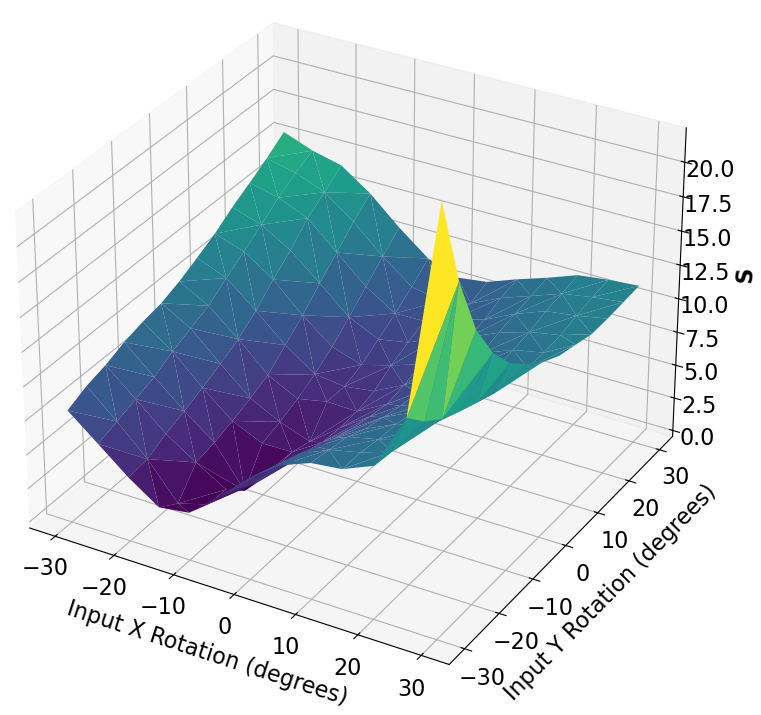
\includegraphics[width=0.3\linewidth]{~/figures/raster/Humeral_dx_sensitivity.png}
	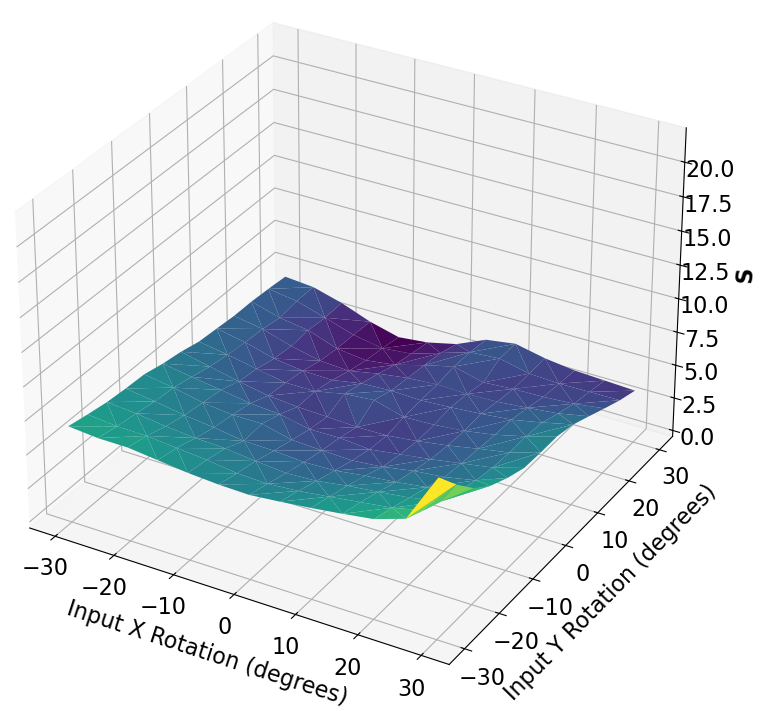
\includegraphics[width=0.3\linewidth]{~/figures/raster/Humeral_dy_sensitivity.png}
	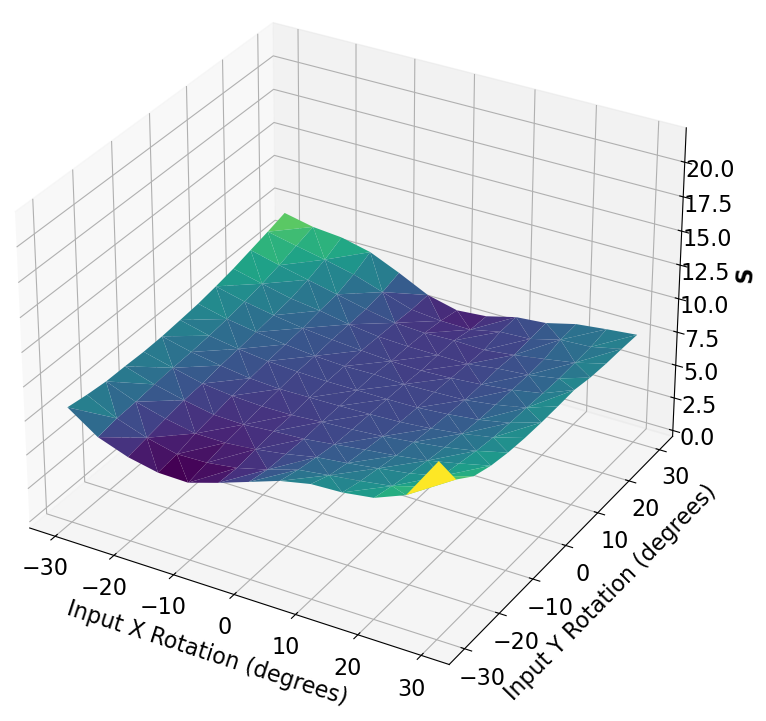
\includegraphics[width=0.3\linewidth]{~/figures/raster/Humeral_dz_sensitivity.png}
	\caption{The $\mathbb{S}$ plot for a humeral implant for $\delta$ rotations along the x, y, and z axis, respectively.}
	\label{fig:hum_sensitivity_plot}
\end{figure}

\begin{figure}[h!]
	\centering
	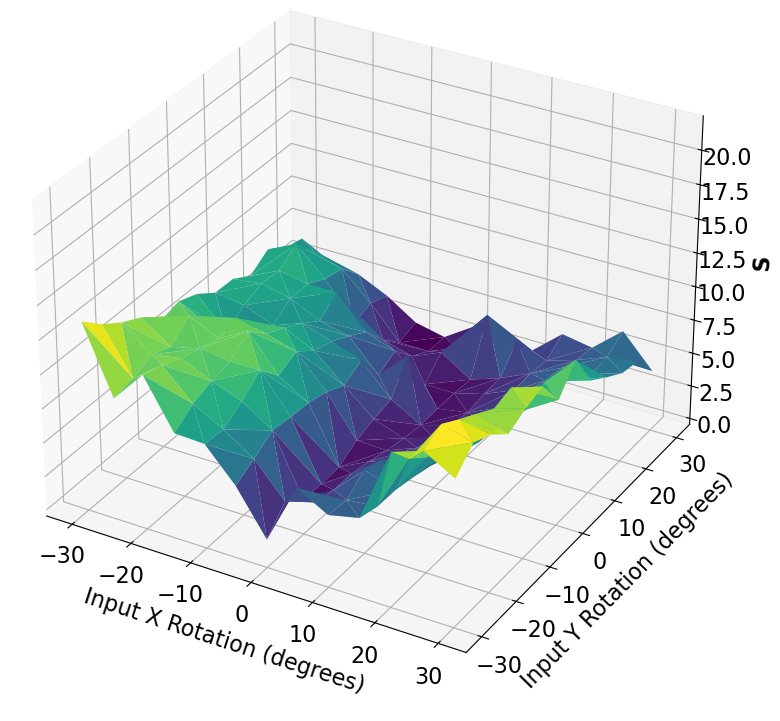
\includegraphics[width=0.3\linewidth]{~/figures/raster/Glenosphere_dx_sensitivity.png}
	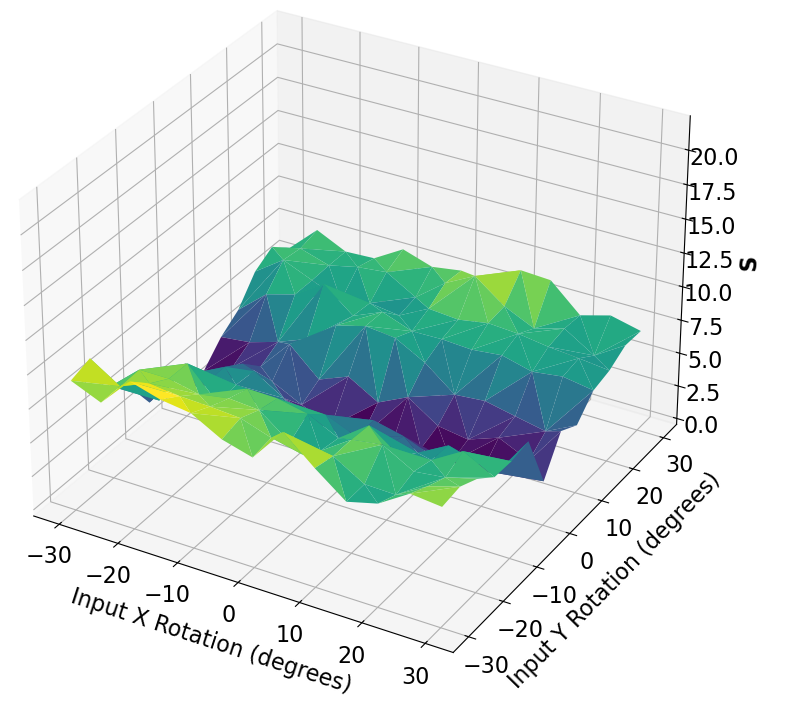
\includegraphics[width=0.3\linewidth]{~/figures/raster/Glenosphere_dy_sensitivity.png}
	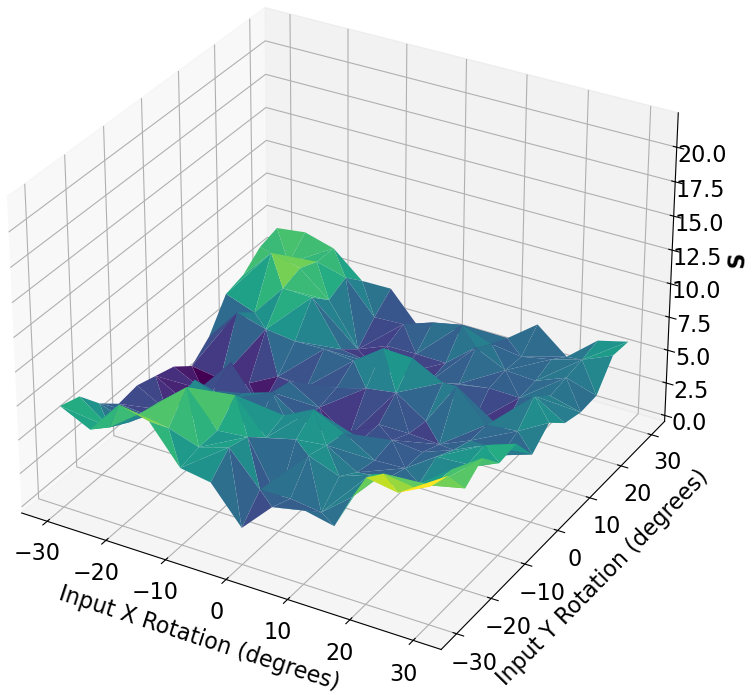
\includegraphics[width=0.3\linewidth]{~/figures/raster/Glenosphere_dz_sensitivity.png}
	\caption{The $\mathbb{S}$ plot for a glenosphere implant for $\delta$ rotations along the x, y, and z axis, respectively.}
	\label{fig:sca_sensitivity_plot}
\end{figure}
\begin{figure}[h!]
	\centering
	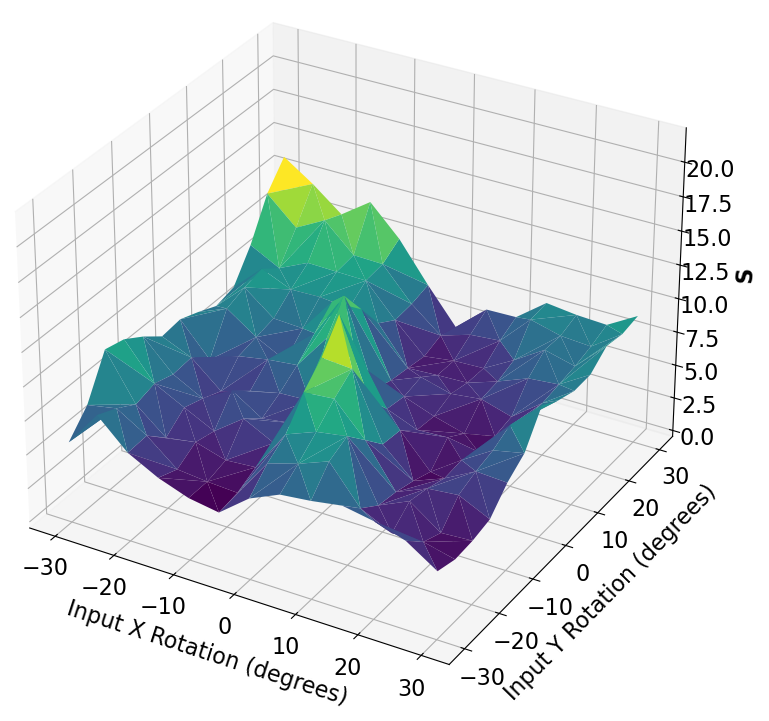
\includegraphics[width=0.3\linewidth]{~/figures/raster/Femoral_dx_sensitivity.png}
	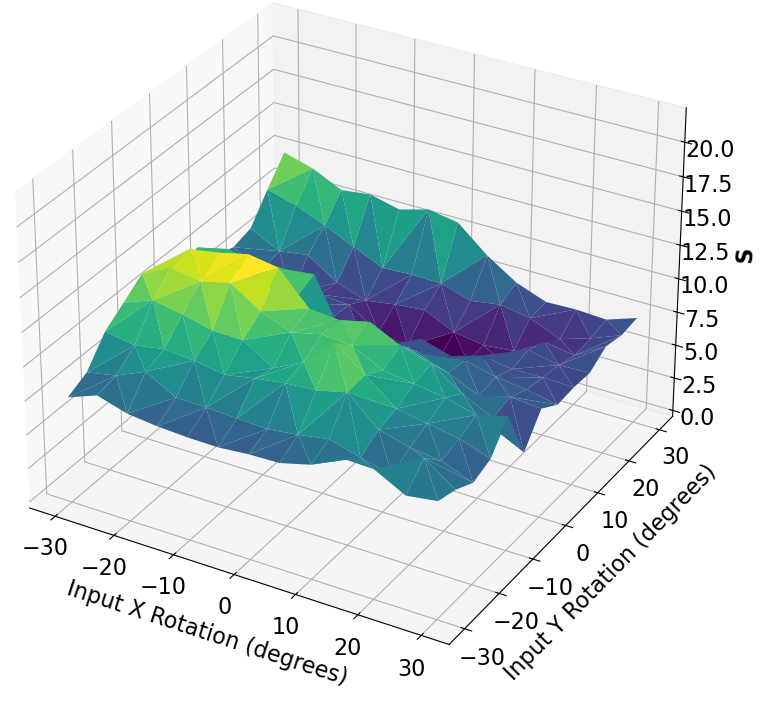
\includegraphics[width=0.3\linewidth]{~/figures/raster/Femoral_dy_sensitivity.png}
	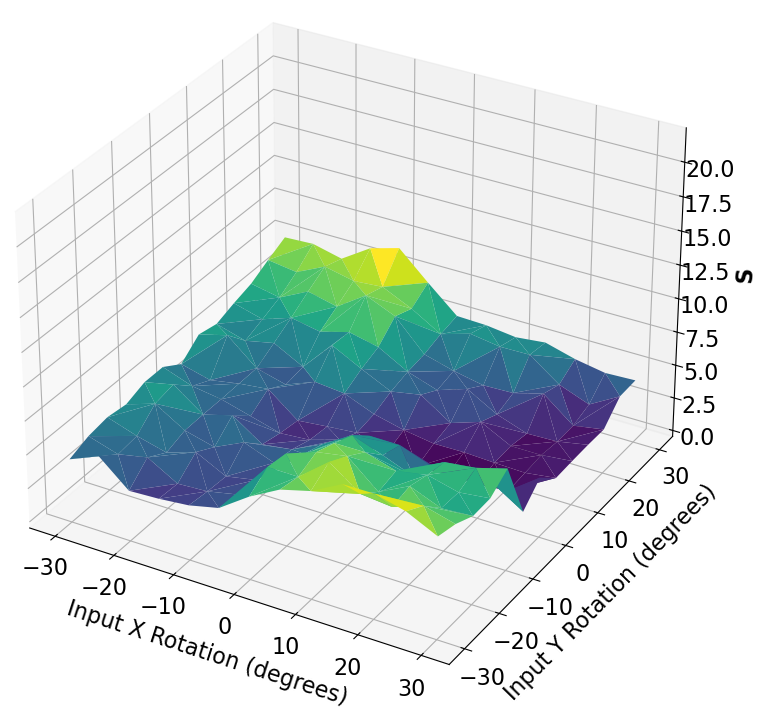
\includegraphics[width=0.3\linewidth]{~/figures/raster/Femoral_dz_sensitivity.png}
	\caption{The $\mathbb{S}$ plot for a femoral implant for $\delta$ rotations along the x, y, and z axis, respectively.}
	\label{fig:fem_sensitivity_plot}
\end{figure}
\begin{figure}[h!]
	\centering
	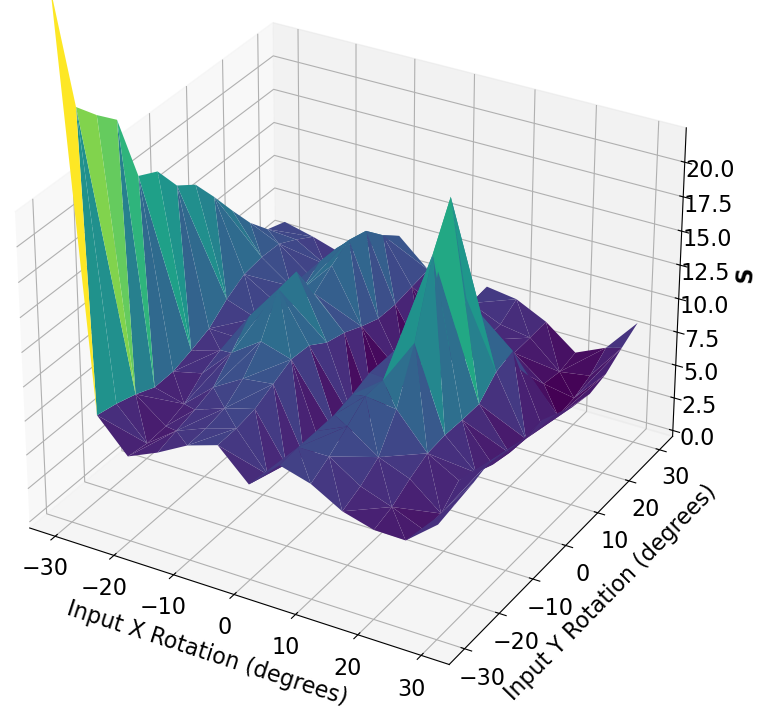
\includegraphics[width=0.3\linewidth]{~/figures/raster/Tibial_dx_sensitivity.png}
	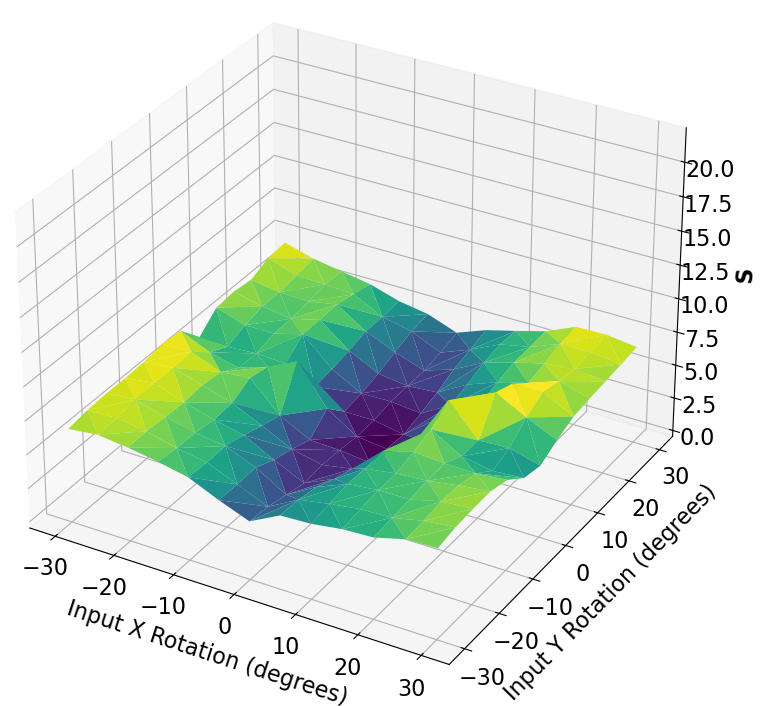
\includegraphics[width=0.3\linewidth]{~/figures/raster/Tibial_dy_sensitivity.png}
	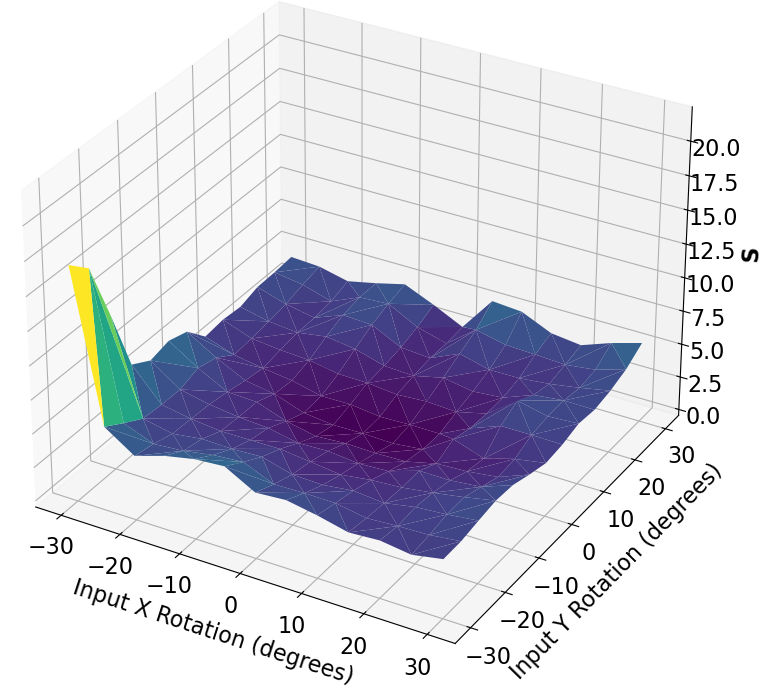
\includegraphics[width=0.3\linewidth]{~/figures/raster/Tibial_dz_sensitivity.png}
	\caption{The $\mathbb{S}$ plot for a tibial implant for $\delta$ rotations along the x, y, and z axis, respectively.}
	\label{fig:tib_sensitivity_plot}
\end{figure}


%%% Local Variables:
%%% mode: latex
%%% TeX-master: "../Jensen_Shape_Sensitivity"
%%% End:
